\documentclass{../pdae} %\documentclass[12pt]{../pdae}
% Necesario aquí para que lea bien el shorttitle
% Título en la cabecera

\shorttitle{Pràctica 4:\\Connexió al Robot}
\title{Creació de les Funcions Bàsiques de Comunicació i d'una Llibreria de
Funcions per Controlar el Robot}

\author{
    Iván Canales\\
    Xavier Ripoll
}

\date{4 de maig de 2018}

\begin{document}
\maketitle

\section{Introducció}

\subsection{Objectius}
% Què es vol fer a la pràctica.

Aquesta pràctica és més oberta que les anteriors. Consisteix en dissenyar una
API per poder controlar el robot, tant les funcions de la interfície com
la seva implementació. Els passos generals són senzills:

\begin{enumerate}
  \item Configurar el port P3 per llegir i enviar dades mitjançant el protocol
        UART.
  \item Crear una funció d'enviament i una altra de recepció a través d'aquest
        port i seguint les especificacions dels motors i sensors AX-*.
  \item Crear un seguit de funcions que actuin com a interfície (API) per poder
        controlar el robot (moure'l, detectar obstacles, sons, etc.) sense
        haver d'interactuar amb el hardware ni els ports directament.
\end{enumerate}



\subsection{Recursos utilitzats}
% Quins recursos del Microcontrolador, Placa d’Experimentació i Robot es fan servir.
De la placa, el \texttt{SMCLK} com a \textit{clock} per controlar
\textit{timeouts} a l'hora d'enviar i rebre paquets, i el port P3 per fer la
comunicació amb els mòduls AX-12 i AX-S1.

Del mòdul AX-12 (els motors), emprem el component principal, que són les rodes.
La nostra API solament disposa de dues funcions per controlar el robot
(\texttt{rotate\_left} i \texttt{rotate\_right}, per moure la roda esquerra i
dreta corresponentment), ja que hem considerat que altres funcions de
desplaçament són molt curtes i compliquen innecessàriament la inferfície.

De l'altre mòdul, el AX-S1 que conté els sensors, emprem el detector de so
i els d'obstacles (dos de laterals i un de frontal). Hem dissenyat funcions
per controlar el nombre de palmades (o cops secs en general) que se senten
i detectar si hi ha obstacles davant del robot.



\subsection{Configuració dels recursos}
% Com s’han configurat els diferents recursos.

\subsubsection{Configuració dels \textit{timers}}

Abans de configurar el \textit{timer}, cridem la funció
\texttt{init\_ucs\_24MHz} per a que inicialitzi el
\textit{unified clock system}.

Usem el \texttt{SMCLK} amb el mode \textit{pull up}, un divisor de freqüència
de valor 8 i una freqüència de 3000 per aconseguir que hi hagi una
interrupció cada mil·lisegon.

\subsubsection{Configuració de la UART}

Per la UART utilitzem també el \texttt{SMCLK}. Per defecte posem la línia en
mode de recepció i la canviarem a enviament solament quan hi hagi un paquet per
enviar, i després la canviarem a recepció de nou.



\subsection{Funcions utilitzades}
% Com i per quines funcions es fan servir.

Aquesta pràctica té un conjunt gran de mètodes que desglossem aquí:

\subsubsection{Inicialitzacions}

Els mètodes \texttt{init\_uart}, \texttt{init\_timers} i
\texttt{init\_interrupts} s'encarreguen de preparar la UART, el \textit{timer}
i les interrupcions, corresponentment.

\subsubsection{\textit{Helpers} pel rellotge}

Hi ha un conjunt de \textit{helpers} encarregats de facilitar l'ús de les
interrupcions de rellotge:

\begin{description}
  \item[\texttt{set\_timer\_interrupt}] Activa/desactiva la interrupció del
    \textit{clock}.
  \item[\texttt{reset\_time}] Posa el comptador del timer a 0.
  \item[\texttt{has\_passed}] Comprova si ha passat un temps donat des que s'ha
    resetejat el \textit{clock}.
\end{description}

\subsubsection{\textit{Helpers} per la comunicació}

Similarment, en tenim per la lectura de dades pel canal UART:

\begin{description}
  \item[\texttt{set\_direction\_rx}] Posa la direcció de les dades en recepció.
  \item[\texttt{set\_direction\_tx}] Posa la direcció de les dades en enviament.
  \item[\texttt{tx\_byte\_uac2}] Envia un \textit{byte} donat.
  \item[\texttt{has\_received\_byte}] Comprova si s'ha rebut cap \textit{byte}
    nou.
  \item[\texttt{get\_read\_byte}] Retorna l'últim \textit{byte} rebut.
\end{description}

\subsubsection{Transmissió i recepció}

Tenim dues rutines principals, \texttt{tx\_instruction} i \texttt{rx\_status}.
La resta de les funcions utilitzen aquestes dues.

\texttt{tx\_instruction} s'encarrega de construir "paquets" de dades que
segueixen el format especificat a la documentació per enviar-los als mòduls
(motors o sensors).

\texttt{rx\_status} realitza la funció contrària: llegeix les dades dels
paquets d'estatus que els mòduls envien cada vegada que cridem
\texttt{tx\_instruction}.



\subsubsection{La interfície}

La nostra interfície disposa de mètodes a diferents nivells. Els dos a més baix
nivell són \texttt{read} (que utilitza la instrucció \texttt{READ\_DATA} dels
mòduls per llegir un o més registres) i \texttt{WRITE\_DATA} que escriu als
registres. La resta de funcions utilitzen aquests dos en comptes de mediar
directament amb \texttt{tx\_instruction} i \texttt{rx\_status}.

Per activar els motors, tenim \texttt{rotate\_left} i \texttt{rotate\_right},
que utilitzen el mètode comú \texttt{rotate\_wheel}. Emprem dos mètodes
diferents en comptes de cridar \texttt{rotate\_wheel} perquè cal invertir la
direcció de rotació en una de les dues rodes per aconseguir que vagin
coordinades.

Per llegir sensors, tenim \texttt{read\_obstacle} (detecta obstacles) i
\texttt{read\_claps} (detecta sons que sobrepassen un cert \textit{threshold}).



\subsection{Problemes}
% Problemes que han sorgit (que no siguin de compilació) i com s’han solucionat.

El principal problema amb el que ens hem trobat ha sigut un a nivell tècnic
relacionat amb la recepció de dades.

Un cop escrites (i provades) les funcions d'enviament (\texttt{tx\_instruction})
i de recepció (\texttt{rx\_status}) de dades, vam provar de construir al
\texttt{main} un bucle infinit que, llegint els sensors, modifiqués la
direcció de moviment del robot.

Va resultar ser, però, que fent-ho així, el programa saltava a una rutina
de captura d'errors genèrics en la que es quedava atrapat. En canvi, posant
interrupcions de 100ms entre iteracions, el problema no succeïa.

Una solució (proposada pel professor) que va funcionar, i amb la que finalment
hem decidit quedar-nos, consisteix en canviar la signatura de
\texttt{rx\_status} perquè, en comptes de retornar un \texttt{RxPacket},
escrigui la informació llegida en una variable global que es pot llegir més
tard en altres punts del programa.



\subsection{Conclusions}

% TODO


\section{Comentari del codi}

% TODO

%\begin{lstlisting}[language=C]
%void Código
%\end{lstlisting}



\section{Diagrames de flux}

% TODO

%\begin{figure}[H]
%  \centering
%  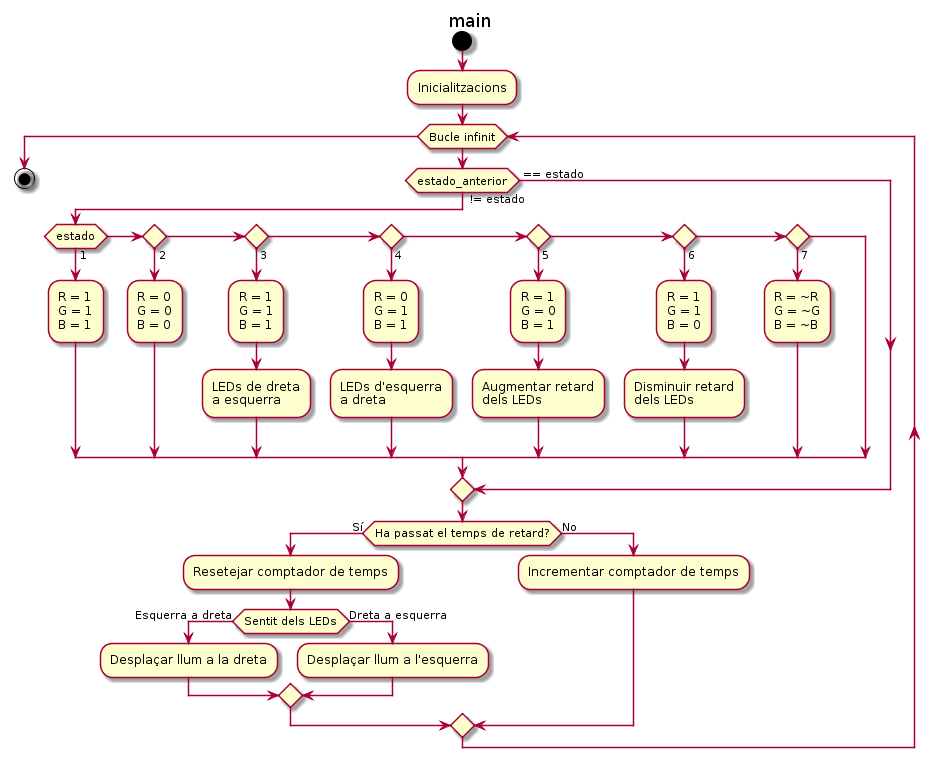
\includegraphics[scale=.45]{main}
%\end{figure}



\end{document}
